\chapter{Introduction}
The goal of this text is to teach mathematical and computer science concepts through a series of stories
designed for students in grades 7-10.

The storyline is similar to the Vikramaditya stories, also called the Vetala tales, in Indian folklore. These stories are believed to have taken place in the 11th century BCE.\footnote{\url{https://en.wikipedia.org/wiki/List_of_Vetala_Tales}}
Collectively, there are 21 stories, one taking place each night. Each story begins with a series of questions, and the protagonist has to successfully answer those questions to set himself free. 


Our stories start on October 31st, Halloween. They take place in a hamlet called Royt, a small college town somewhere in Upstate New York. Royt was a prosperous town a hundred years ago, but these days the town has many dilapidated buildings and a rather imposing cemetery. Ajur and his parents live in this hamlet. Ajur has a pet dog named Jura, who accompanies Ajur wherever he goes.  In the cemetery lives Rishnak, a ghost, who was a tyrant but now has good intentions.

\section{Characters}

\textbf {Ajur} - A young boy who is interested in mathematics but easily gets bored.\\
\noindent
\textbf {Jura} - Ajur's pet dog.\\
\noindent
\textbf{Kinaja} - An angel who helps Ajur overcome challenges posed by Rishnak.\\
\noindent
\textbf{Rishnak} - A ghost with a mathematical bent of mind from whom Ajur wants to escape by solving various mathematical challenges.\\
%%\noindent
%%\textbf{Royt} - The hamlet in which the entire story takes place, home of the most famous cemetery in the country.

\section{Notation}
\textbf{Graphs} \index{Graphs}, also known as networks \index{networks}, occur naturally in many different applications. They are abstractions of a relation between any two objects, i.e.,~a binary relation. Objects can, for example, be people, cities, countries, or webpages. These objects are represented by \textbf{vertices}, \index{vertices} usually drawn as dots 
or circles on a page. Relations may exist between any two different objects. These relations are represented as lines connecting the two vertices and are called \textbf{edges} \index{edges}.

We will illustrate with three examples. In our first example [Figure~\ref{1g1}], there are four vertices representing objects, the numbers~0, 1, 2, and~3. There are six relations (or edges); these relations are \{0,1\}, \{0,2\}, \{0,3\}, \{1,2\}, \{1,3\}, and \{2,3\}. These relations are symmetric, meaning if there is a relation between vertex~0 and vertex~1, then there is also a relation between vertex~1 and vertex~0. Such graphs are called \textbf{undirected} \index{undirected graph} graphs.
\begin{figure}
\begin{center}
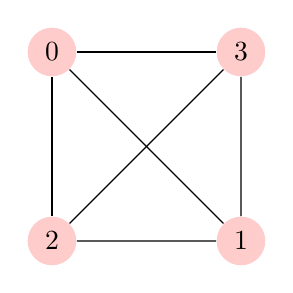
\begin{tikzpicture}
  [scale=.6,auto=left,every node/.style={circle,fill=red!20}]
  \node (n1) at (0,0) {0};
  \node (n2) at (4,-4)  {1};
  \node (n3) at (0,-4)  {2};
   \node (n4) at (4,0)  {3};

  \foreach \from/\to in { n1/n2,n1/n3,n1/n4,n2/n3,n2/n4,n3/n4}
    \draw (\from) -- (\to);

\end{tikzpicture}
\caption{A graph with four vertices and six edges}\label{1g1}
\end{center}
\end{figure}
\begin{newpage}
\end{newpage}

In our next example [Figure \ref{1g2}], we have five vertices representing five people, namely Bob, William, James, Chris, and Ajur. The edges in the graph represent friendship. Chris is friends with William, James, and Ajur. Bob is friends with William and James. These friendship relations are depicted as a graph with five vertices and five edges.
\begin{figure}
\begin{center}
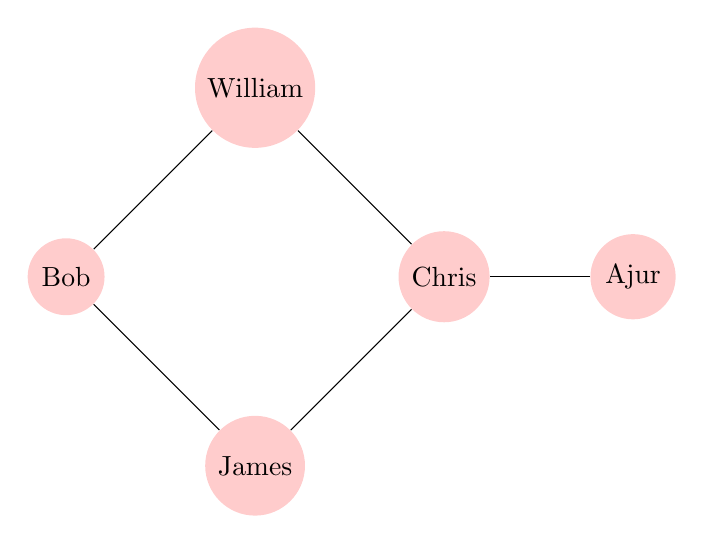
\begin{tikzpicture}
  [scale=.6,auto=left,every node/.style={circle,fill=red!20}]
  \node (n1) at (0,0) {Bob};
  \node (n2) at (4,4)  {William};
  \node (n3) at (4,-4)  {James};
   \node (n4) at (8,0)  {Chris};
    \node (n5) at (12,0) {Ajur};
  \foreach \from/\to in { n1/n2,n1/n3,n3/n4,n2/n4,n4/n5}
    \draw (\from) -- (\to);

\end{tikzpicture}
\caption{A friendship graph with five vertices and five edges}\label{1g2}
\end{center}
\end{figure}


\begin{newpage}
\end{newpage}
In our third example [Figure \ref{1g3}], we have seven Northeastern states in the United States, namely New York (NY), Connecticut (CT), Vermont (VT), Maine (ME), Massachusetts (MA), Rhode Island (RI), and New Hampshire (NH). The relationship represented in this graph is the sharing of a border with another state. Therefore, NY borders CT, VT, and MA. CT additionally borders RI and MA. VT additionally borders MA and NH. ME only borders NH. MA additionally borders RI and NH. These state-border relations are depicted as a graph with seven vertices and 10 edges.

\begin{figure}
\begin{center}
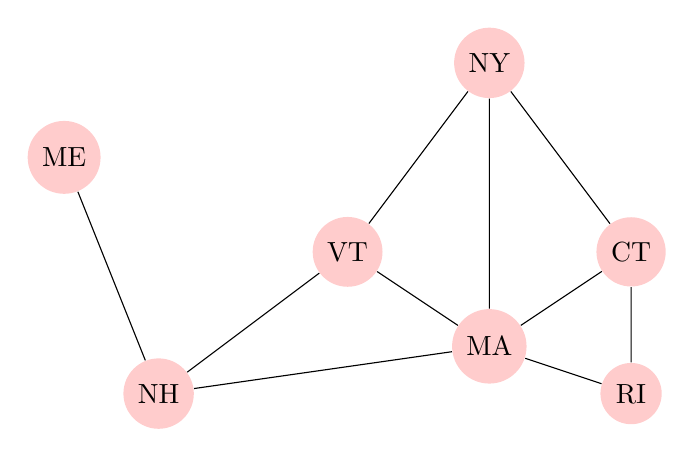
\begin{tikzpicture}
  [scale=.6,auto=left,every node/.style={circle,fill=red!20}]
  \node (n1) at (0,1) {ME};
  \node (n2) at (2,-4)  {NH};
  \node (n3) at (6,-1)  {VT};
   \node (n4) at (9, -3) {MA};
   \node (n5) at (9,3)  {NY};
    \node (n6) at (12,-1) {CT};
    \node (n7) at (12, -4) {RI};
  \foreach \from/\to in { n1/n2,n2/n3,n2/n4, n3/n4,n3/n5,n4/n5,n4/n6,n4/n7,n5/n6,n6/n7}
    \draw (\from) -- (\to);

\end{tikzpicture}
\caption{A graph representing seven Northeastern states in the United States, with seven vertices and 10 edges}\label{1g3}
\end{center}
\end{figure}

One other term to introduce here. If there is an edge between two vertices (e.g.,~between NY and VT in Figure~\ref{1g3}), we say that these two vertices are \textbf{adjacent}. More specifically, NY is adjacent to VT. And VT is adjacent to NY.

%\chapter{Introduction}
   

\chapter{A Trip to the Cemetery}
It was Halloween, a cold and dreary fall afternoon. Ajur was interested in visiting the famous cemetery in Royt as any teenager with an adventurous spirit would be wont to do. His pet dog Jura, a Labrador, was eager to follow. As Ajur examined the old headstones, he lost track of time, and it grew dark. He felt tired, so he and Jura sat under a tree and fell asleep.

Deep in sleep, they were awakened by a loud noise. The noise was from Rishnak, a ghost who lived in the cemetery. Rishnak had died many years ago; he used to teach mathematics and graph theory to talented high school students all throughout the area. When Rishnak spotted Ajur in the cemetery, he thought to himself, ``Here is an unusual teenager.'' Perhaps he could test whether this youngster was proficient in mathematics. And if he was indeed proficient, Rishnak could reward him with his magical powers. When Rishnak appeared in front of Ajur, Jura jumped up and started barking. Ajur sat up with a start.

Rishnak was afraid he would intimidate Ajur by being brusque. Jura's barking became louder and louder, so Rishnak started talking in a soft voice. He gently asked what grade Ajur was in. Ajur replied that he was in the 8th grade. Rishnak asked what subjects Ajur liked most in school, to which Ajur proudly said, ``mathematics.'' Rishnak smiled. He told the boy that he had been cursed to live as a ghost, and his curse could only be lifted if he could reward a youngster who could answer all of his questions.

Ajur was intrigued by Rishnak's plight. Standing up now, Ajur was excited for the possibility of rewards and the opportunity to help lift the curse on Rishnak, a poor ghost. Ajur also thought he would be able to tell his friends about his adventure.